\section{Baseline}\label{sect:baseline} 

The baseline algorithm defined in this study is a standard genetic algorithm (GA)~\cite{mitchell1998introduction} that is used to optimize 
process allocation in cloud computing environments. The idea is that by optimizing the process allocation, the energy consumed by the cloud envirnoment is minimized as well.
The GA is a stochastic population-based search algorithm that is based on the principles of natural selection and genetics.
It is a meta-heuristic that is used to find approximate solutions to optimization problems.~\cite{kramer2017genetic}

The GA is composed of the following components:
\begin{itemize}
    \item A population of candidate solutions;
    \item A fitness function that is used to evaluate the quality of each candidate solution;
    \item A selection operator that is used to select candidate solutions for reproduction;
    \item A crossover operator that is used to combine the selected candidate solutions to produce new candidate solutions;
    \item A mutation operator that is used to introduce random changes to the candidate solutions;
    \item A termination criterion that is used to determine when the GA should stop searching for solutions.
\end{itemize}

\begin{figure}[h]
    \centering
    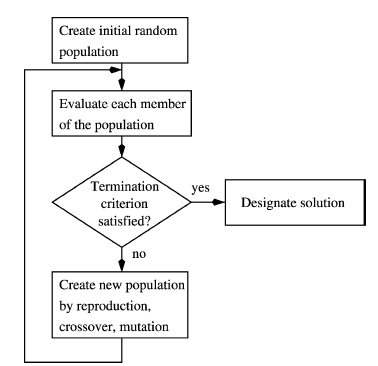
\includegraphics[width=0.5\textwidth]{./resources/examples/GAWorkflow.png}
    \caption{How a Genetic Algorithm works.}
    \label{fig:baseline}
\end{figure}
How a Genetic Algorithm (GA) works is shown in the flowchart~\cite{GAWorkflow} shown in Figure~\ref{fig:baseline}.

In this setting, the candidate solutions are represented by a list of tuples, each of which contains a Server and a list of Processes.
The initial population is generated by iterating over the Server list. 
For each Server, from the list of all the Processes, iteratively, a process is selected at random with probability $$p = \frac{1}{n}$$
with $n$ being the number of servers taken into account in the solution. As a Process is selected, it is removed from the global Process list.\\

Then, the fitness function~\eqref{fitness}, is used to evaluate the quality of each candidate solution.

% Discuss about the parameters of the GA
The baseline genetic algorithm has been tested over a pletora of parameters, in order to find the best combination that would lead to acceptable results.
The parameters that have been tested are:
\begin{itemize}
    \item The probability of selecting a process for a server;
    \item The crossover rate;
    \item The probability of mutation;
    \item The population size;
    \item The number of generations.
\end{itemize}

The selection probability $p_s$ is equal to $\frac{1}{\#_{servers}}$. In the first settings of the experiments this value was 
set in different ranges between $[0.3, 0.6]$, but this not only led to a very slow convergence of the GA but produced undesired noise
in the results in most of the experiments.
The crossover rate $p_c$ is set to $0.9$. A starting value of $0.5$ was used, but this led to unsatisfactory results, opposed to what~\cite{mirjalili2019genetic} claimed
in their research.
Better results were obtained by increasing the crossover rate to $0.7$, but the best ones were yield by $p_c = 0.9$, supported by~\cite{hassanat2019choosing}.
The probability of mutation $p_m$ has been initially tested in the range $[0.1, 0.3]$. However, as found in previous research works,
a mutation rate over $0.01$ is a synonym of heavy noisy training epochs and close to no convergence. In fact, it has been found that 
the optimal values for the mutation rate ranges in $[0.005, 0.05]$ for a population size $s_p$ between $100$ and $200$ individuals.~\cite{patil2015optimal}
It follows that the chosen parameters for the mutation rate are $p_m = 0.01$ and $s_p = 200$.

As for the number of epochs employed, for both hardware constraints and time reasons, the GA has been run for a maximum of $500$ generations.
For each experiment, the GA is run $10$ times and the results are averaged in order to obtain an insightful overlook of the performances.

The baseline algorithm has been created to be initially compared to a greedy assignation method of simple ideation.
The fitness function employed in the baseline algorithm has been used to compare the results between the greedy method and the baseline algorithm.
\ecomment{Compare the greedy and the baseline algorithm.}

% include the graphics
\begin{figure}[h]
    \centering
    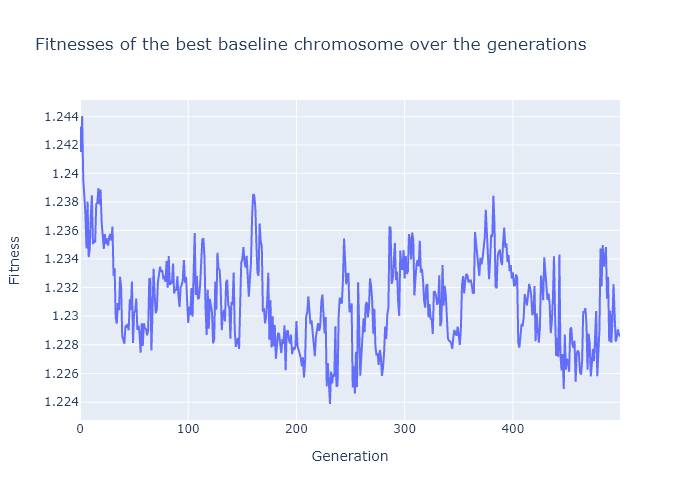
\includegraphics[width=0.5\textwidth]{../../../Code/Genetic/results/baseline/graphs/pop_size_200/500_epochs/average_fitness.png}
    \caption{The average of the Baseline Algorithm over $500$ epochs}
    \label{fig:average_baseline}
\end{figure}

As it can be seen from the results in Figure~\ref{fig:average_baseline}, the fitness function evaluated with the baseline algorithm shows promising results
in a time range comprised between $200$ and $250$ epochs, with its minimum at $230$.
\ecomment{Insert the maximum value from the starting point, the minimum value and the corresponding epoch.}

\ecomment{Discuss about the results of the greedy algorithm}